\documentclass[ngerman,onecolumn,bibliography=totocnumbered]{scrreprt}

% Spracheinstellungen
\usepackage[T1]{fontenc}
\usepackage{lmodern}
\usepackage[utf8]{inputenc}
\usepackage{babel} % Sprache als Klassenoption übergeben

% Mathematik
\usepackage{mathtools} % Verbesserungen zu amsmath.sty
\usepackage{amsfonts}
\usepackage{amssymb}
\usepackage{physics}
\usepackage{braket}
\usepackage[version=3]{mhchem}
\usepackage{tikz-feynman}

\newcommand{\mup}[1]{\textnormal{#1}} % nicht-kursiver Text z.B. in Subscripts
\newcommand{\I}{\mup{i}} % imaginäre Einheit
\newcommand{\E}{\mup{e}} % Eulersche Zahl
\newcommand{\vect}[1]{\vec{#1}} % 3-Komponentiger Vektor
\newcommand{\mperiod}{\,\text{.}} % Satzzeichen in Formeln
\newcommand{\mcomma}{\,\text{,}}

% Typografie
\usepackage{microtype} % Mikrotypografie wie überhängende Interpunktion
\usepackage{csquotes} % tolle Anführungszeichen
\usepackage{booktabs} % Tabellen
\usepackage{caption} % Float-Beschriftungen
	\captionsetup{
		margin     = 10pt,
		font       = small,
		labelfont  = bf,
		figurename = {Fig.},
		tablename  = {Tab.}
	}
\usepackage{subcaption} % Unterabbildungen
\makeatletter
	\g@addto@macro\bfseries{\boldmath} % Bold math in headings
\makeatother
%Table of Contents
\usepackage[nottoc,notlof]{tocbibind} %Einbinden Bibliography in Table of Contents

% Grafiken
\usepackage{graphicx}
% \usepackage{placeins}
\usepackage{siunitx} % Zahlen, Einheiten und Tabellenformatierung
	\sisetup{
		locale = DE,
		per-mode = symbol,
		output-decimal-marker = {.},
		separate-uncertainty = true,
		binary-units = true
	}
	\DeclareSIUnit\year{a}
	\DeclareSIUnit\pixel{px}
	\DeclareSIUnit\line{line}
\graphicspath{{./images/}}
\usepackage{scrlayer}
\DeclareNewLayer[% define a new layer
  foreground,
  textarea,
  contents={\parbox[b][\layerheight][b]{\layerwidth}{%
		\centering
    
\includegraphics[scale=0.5]{uni-seal.png}
  }}
]{titlepage.seal}
% Dokumenteinstellungen
\usepackage{pdfpages}
\usepackage{scrlayer-scrpage} % Änderung der Kopf-/Fußzeile%
% %\usepackage{scrpage2}
\usepackage{lastpage} % lässt auf die Seitenanzahl zugreifen
% \renewcommand{\baselinestretch}{1.5}
% \usepackage{geometry}
% \geometry{top=2.5cm, left=2.5cm, right=3cm, bottom=3.5cm}

% macht das abbildungsverzeichnis nummeriert
\patchcmd{\listoffigures}{\chapter*}{\chapter}{}{}

% Bibliographie
\usepackage[backend=bibtex,hyperref=true]{biblatex}
	% TODO Warum steht der Literatur-Section-Name in der Kopfzeile?!
	\addbibresource{Bib/Full_Bibliographie.bib}
%\bibliography{Bib/GenomicPrediction.bib}

\usepackage{hyperref}

\pagestyle{scrheadings}	% sagt Koma-Skript, dass selbstdefinierte Kopfzeilen verwendet werden
\typearea{16} % stellt Seitenspiegel ein
%\columnsep25pt % definiert Breite zwischen den zwei Spalten von \twocolumns

\renewcommand{\pnumfont}{\normalfont\rmfamily\slshape} % ändert die Schriftart der Seitennummerierung

%Bsp Makros
%\newcommand{\teachm}{\emph{teach'm tool} }
% \newcommand{\orb}[2]{\(\text{#1}_\text{#2}\)}
% \newcommand{\xsys}{\(\text{x}^2{-}\text{y}^2\)}
% \newcommand{\zs}{\(3\text{z}^2-\text{r}^2\)}
% \newcommand{\cre}{{\dag}}
% \newcommand{\ann}{{\vphantom{\dag}}}
% \newcommand{\psibar}{{\bar{\psi}}}
% \newcommand{\Dp}[1]{\text{d}\psi_{#1} }
% \newcommand{\Dpb}[1]{\text{d}\psibar_{#1} }
% \newcommand{\DPP}[1]{\text{d}\psibar_{#1} \text{d}\psi_{#1} }
% \newcommand{\D}[1]{\text{d}{#1}\text{ }}
% \newtheorem{definition}{Definition}

%Einstellungen zur Titelseite
\begin{document}
\titlehead{\centering
\includegraphics[scale=0.4]{CCTB_Logo.pdf}}
\title{Selection on loss-of-function variants}
\subject{Master Thesis}
\subtitle{\vspace{1cm}Master Biosciences \\ Faculty of Biology \\ Julius-Maximilians-Universität Würzburg}
\author{submitted by Laura Steinmann \\from Würzburg\\ Supervisor PD Arthur Korte}

\date{\today}
\pagenumbering{roman}


\AddLayersToPageStyle{empty}{titlepage.seal}% add the layer to pagestyle empty
\maketitle
\thispagestyle{empty}
\RemoveLayersFromPageStyle{empty}{titlepage.seal}
\newpage
\vspace*{\fill}
\begingroup
\centering
\textsf{\textbf{Supervisor} \quad PD Arthur Korte}\\
\vspace{2cm}
\textsf{\textbf{Second reviewer} \quad Prof. Dr. Dirk Becker} \\
\vspace{2cm}
\textsf{\textbf{Date of Submission, office stamp}}\\
\vspace{10mm}
\_\_\_\_\_\_\_\_\_\_\_\_\_\_\_\_\_\_\_\_\_\_\_\_\_\_\_\_\_\_\_\_\_\_\_\_\_\\
\endgroup
\vspace*{{\fill}}
\setcounter{page}{1}
\chapter*{Zusammenfassung}
%TODO HIER KOMMT DAS ABSTRACT IN GERMAN
\chapter*{Abstract}
%TODO HIER KOMMT DAS ABSTRACT IN ENGLISH
\newpage
\tableofcontents
\pagenumbering{arabic}
% !TeX root = main.tex
\chapter{Introduction}
To survive in an ecosystem organisms need to adapt to the specific abiotic and biotic factors around them. This is particularly important for plants since they can not change their habitat during their lifespan. Adaptation can operate on different levels of the organisms from the adaptation of protein function to modifications in cell functions or whole tissue functions. But the underlying fundamental process that drives adaptation is the modification of the genetic material DNA.\\
Modifications on DNA level are called mutations and in four different groups. In the following description we consider just mutations which occur in coding regions of the genome although they can be distributed throughout all regions of the genome. A point mutation, which is the first group of mutations and can be also called single nucleotide polymorphism (SNP), is concerning just one single base pair. These changes the DNA sequence on one single point and therefore lead to changes of the transcribed mRNA. The second class of mutations are insertions. These insert a new sequence into the former DNA sequence and thus elongate it. These insertions can have a variety of length from one single bp to a few hundred bp and even longer sequences can be added.  The contrasting class of insertions are deletions, which lead to a reduction of base pairs in a variety of lengths in the former DNA strand. The last category of mutations are duplications. As implied by the name, regions of the DNA get duplicated and inserted at a different position. The regions can be copied abnormally one or even more times.\\
These mutations are first of all just changes in the DNA but indirectly they impact all the resulting processes. The DNA first gets transcribed into mRNA. This process is not affected by the evolved mutations. But after the transcription the mRNA gets translated into proteins. In this step the impact of the mutations appear since a triplet codon gets translated into a specific amino acid, which can change due to the mutation in the DNA as postulated by Gamow\cite{crick1988}. The mutations can have different effects on the resulting protein. The insertions or deletions lead mostly to a shift in the reading frame and therefore change the sequence of amino acids in a wide range. Point mutations, although they change just a single codon, can have different effects on the translated amino acid and therefore on the functionality of the resulting protein. As it was known that 23 amino acids exists and when the knowledge arises that a codon includes three base pairs the genetic code could get deciphered by \textcite{Nirenberg1965}. The gain of knowledge deciphering this genetic code showed that the genetic code is degenerated as identified by \textcite{Lagerkvist1978}, which means that not one codon is directly linked to an amino acid rather that there are multiple codons that can initiate the same amino acid, which is showed in \autoref{fig:Codons} a). For the topic of point mutations we have three possible outcomes resulting after such mutation. The first outcome is a synonymous mutation, which is the less severe one and does not change the protein at all. Here a base pair changes but the translated codons provoke the same amino acid. An schematic representation of synonymous mutations can be found in \autoref{fig:Codons} b). As shown in \autoref{fig:Codons} c) a mutation could also be a non-synonymous mutation where the modified codon leads to an exchange of the amino acid type. The prediction of how severe these non-synonymous mutations are is hard to do without further analysis. It depends on many circumstances for example if the location is a catalytic region or to which other amino acid it is exchanged. Such a mutation can be very unnoticeable or on the other hand making the protein non-functional. The last kind of point-mutations are premature stop codons. They represent a mutation of a usual codon to a stop codon as it can be seen in \autoref{fig:Codons}d). This means most of the time drastic changes in the protein functionality since the resulting protein is truncated. Thereby premature stop codons represent the most interesting kind of mutations for understanding adaptation in plants since they can be recognized in the DNA level and they should change the function of the truncated protein.\\
\begin{figure}[tb]
    \centering
    \begin{minipage}[h]{0.9\textwidth}
      \centering
      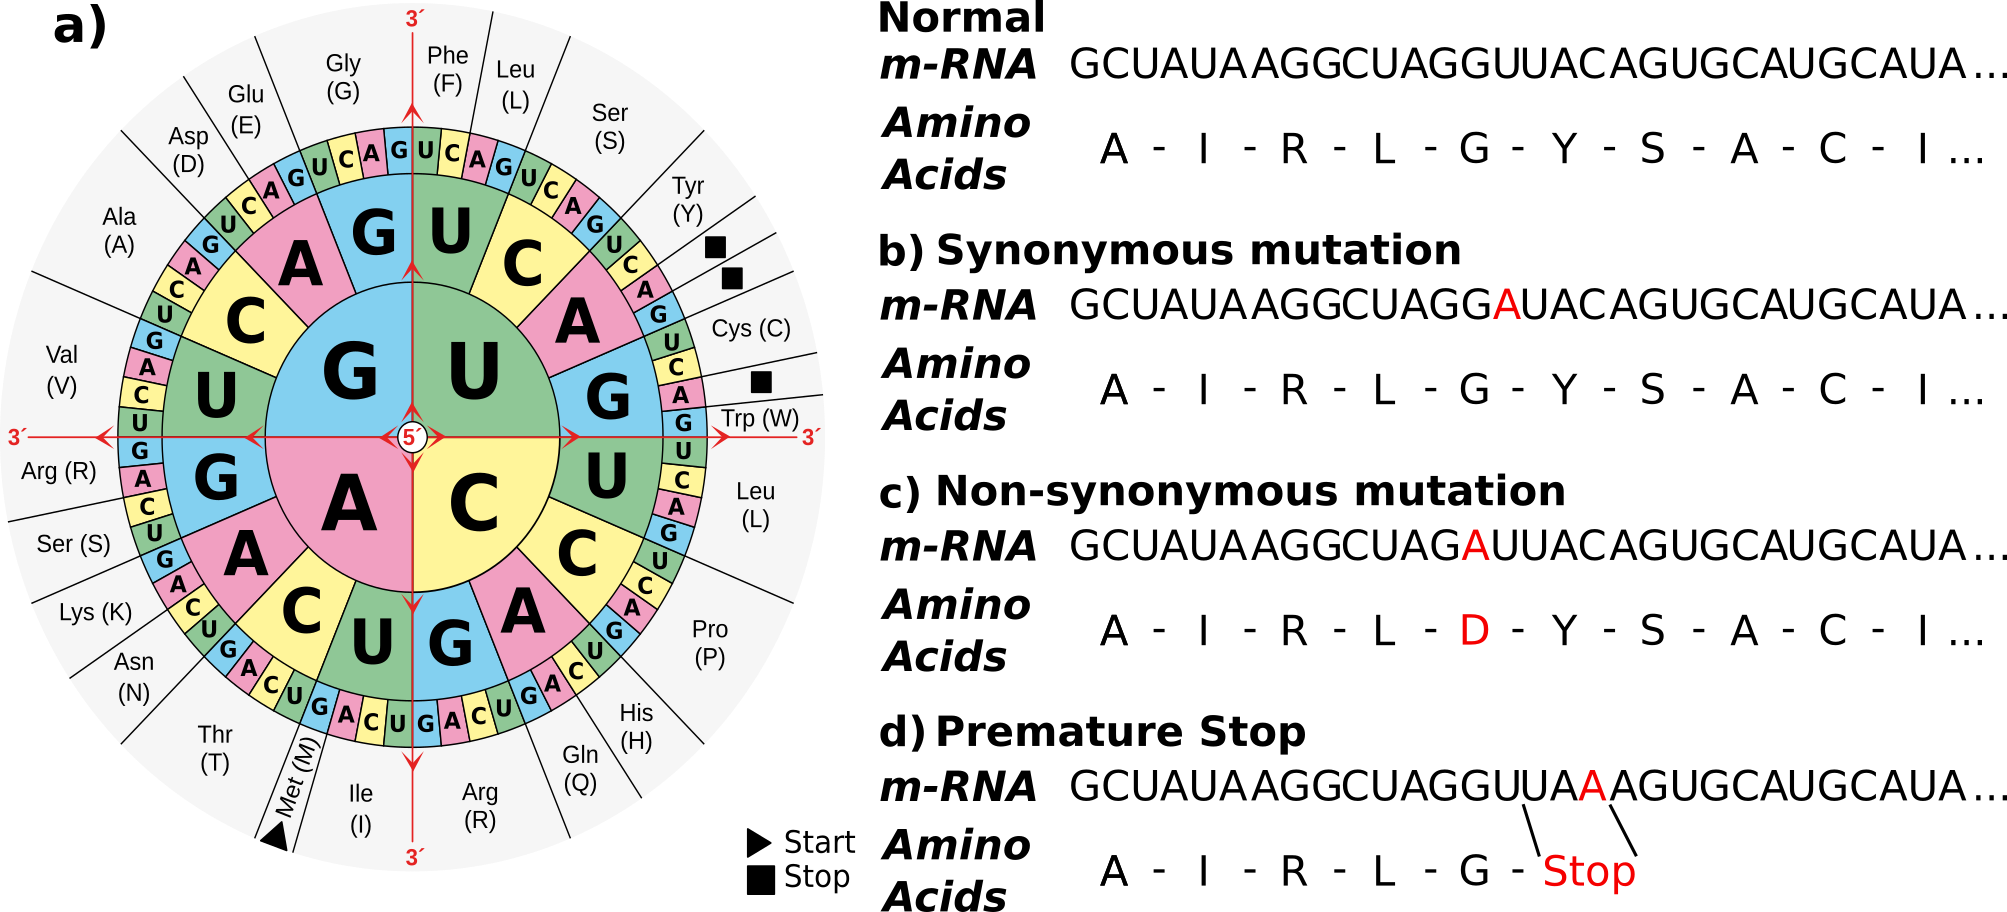
\includegraphics[width=1\textwidth]{images/Mutations.png}
      \caption{\textbf{Schematic representation of point mutation classes}\\
      a) The genetic code (image taken from \textcite{bresch2013}); b) A schematic representation of a synonymous mutation, which affects the mRNA but not the amino acid sequence. c) A schematic representation of a non-synonymous mutation. The change of a single base pair in the mRNA sequence changes to an exchange of the amino acid type. d) A schematic representation of a premature stop codon. Retrieved from a exchange of a single base pair an premature stop codon appears and stops the amino acid sequence.}
     \label{fig:Codons}
    \end{minipage}
  \end{figure}
Until recently in evolutionary theories the axiom exists that these described mutations occur randomly throughout the genome and that solely after occurrence of mutations the evolutionary selection operates and shapes the genetic pool of a population\cite{futuyma1986}. From this axiom it can be deduced that natural selection acts on this mutations by classifying fatal modifications and filter these out of the genetic pool. The time span during which this genetic pool adapts to a single mutation is depending on the severity of the modification. That also implies that mutations which have a neutral significance like synonymous mutations are not shaped by the selection force. On the other side positive impact is reinforced by the selection force so that these mutations get accumulated in the genetic pool.\\
If one now only considers the mutation type premature stop codons some hypotheses can be used to explain the effects of mutations on gene regulatory networks. Since the occurence of premature stop codons is leading directly to a loss of function in this protein one can consider that the evolutionary selection force stabilizes the gene regulatory networks by maintaining the diversion of this networks. Practically this means that if a protein is knocked out by a premature stop codons the pathways around this gene are getting more important and you expect that they are under a high conservation force by evolutionary selection and selection prevent a accumulation of premature stop codons in the rest of the gene regulatory network.\\
In our following project we want to study the attributes and occurence of these premature stop codons. We want to characterize how the natural selection is shaping population structures through generating loss-of-function variants and how they affect the adaptation process of organisms. We therefore follow a bioinformatical approach by applying data analysis and statistical algorithms on different genomic data and with these try to find evolutionary patterns. 
\newpage
% !TeX root = main.tex
\chapter{Material}
In this chapter we will have a look at the necessary computing infrastructure and the code base that I developed for studying of the selection on loss-of-function variants. At the end of this chapter we will have a look at our used dataset.
\section{Computational Material and Resources}
In this section I will explain the computational material. We will start with the computing infrastructure we used for our analysis and continue with looking at the location and dependencies of our code base.
\subsection{Computing Infrastructure}
The whole analysis is calculated on the institutes own high-performance computer cluster. With access to a computer node with 80 cores and 512 GB RAM. Also not all analysis need the maximum capacity of this computer node especially working with the basic unfiltered dataset consums a lot of RAM. To recapitulate any analysis access to a high-performance computer node is therefore necessary. 
\subsection{Code Base}
To study how premature stop codons get distributed in the genetic pool and shape the adaptation in plants we followed a completely bioinformatical based approach. Therefore we developed the statistical analysis and the data analysis in programming languages. To follow these ideas use mainly python but also R as an additional language to complete the workflow set up on an linux based system (Debian). If you like to recapitulate the analysis you can find the code in a github repository \url{https://github.com/laurasteinmann/Premature_Stop_Codons.git}.\\
Although at the moment there are no strict dependency on software versions I will list the used packages and there versions since there is the possibility of semantic changes in future versions. For the Python analysis part we use python (3.10) and the important packages for dealing with numerical data and big data analysis like pandas (1.4) and  numpy (1.22). For calculating statistical test we use scipy (1.8.0). For visualizing our results we use the matplotlib package (3.5), the seaborn package (0.11) and the matplotlib\_venn package (0.11). For dealing with genomic data and filtering it we use the R language with version 4.1.3 and the vcfR library (1.12)
\section{Dataset of 1001 Genomes Project}
\chapter{Methods}
\newpage
% !TeX root = main.tex
\chapter{Results}
By studying the attributes and the occurrence of premature stop codons in the 1,135 population of \textit{A. thaliana} we try to characterize how natural selection is shaping population structures through loss-of-function variants. To answer this research question we followed an statistical workflow. We will start the project by establishing the distribution of premature stop codons in the 1,135 accessions of \textit{A.thaliana} dataset and continue by generating two high confidential datasets for our further analysis. Here we will follow two separate approaches. The first is based on the gene expression differences between wildtype and knock-out accessions. The second selects stop codons based on the calculation of the remaining length of the protein. Finally we  investigate the interactions between premature stop codons and finish our analysis comparing a control group of mutations, which will be the synonymous mutations. 
\section{Distribution of premature stop codons in \textit{A. thaliana}}
\label{sec:Distribution_Results}
As a starting point for understanding how selection influences premature stop codons in populations of \textit{A. thaliana} we analyse the distribution of premature stop codons. In the 1,135 population of \textit{A. thaliana} we observe 29029 premature stop codons distributed over the whole genome and population. Since we need additional information on gene expression patterns we focus our further analysis on the 665 population, which represents the overlap of accessions with genomic and transcriptomic information. In the population of 665 accessions of \textit{A. thaliana} we find hundreds of premature stop codons in each accession, which is shown in \autoref{fig:Distribution_Premature_Stop_Codons_all} a). The only exception is the col-0 (138) accession, which is by definition the reference genome and does not contain any mutations. Besides that all other accessions do have several hundred premature stop codons up to an maximum accession, which includes over 1023 premature stop codons. On average an instance of the 665 \textit{A. thaliana} accessions contains 671 premature stop codons distributed throughout its genome.

\begin{figure}[tb]
    \centering
    \begin{minipage}[h]{0.9\textwidth}
      \centering
      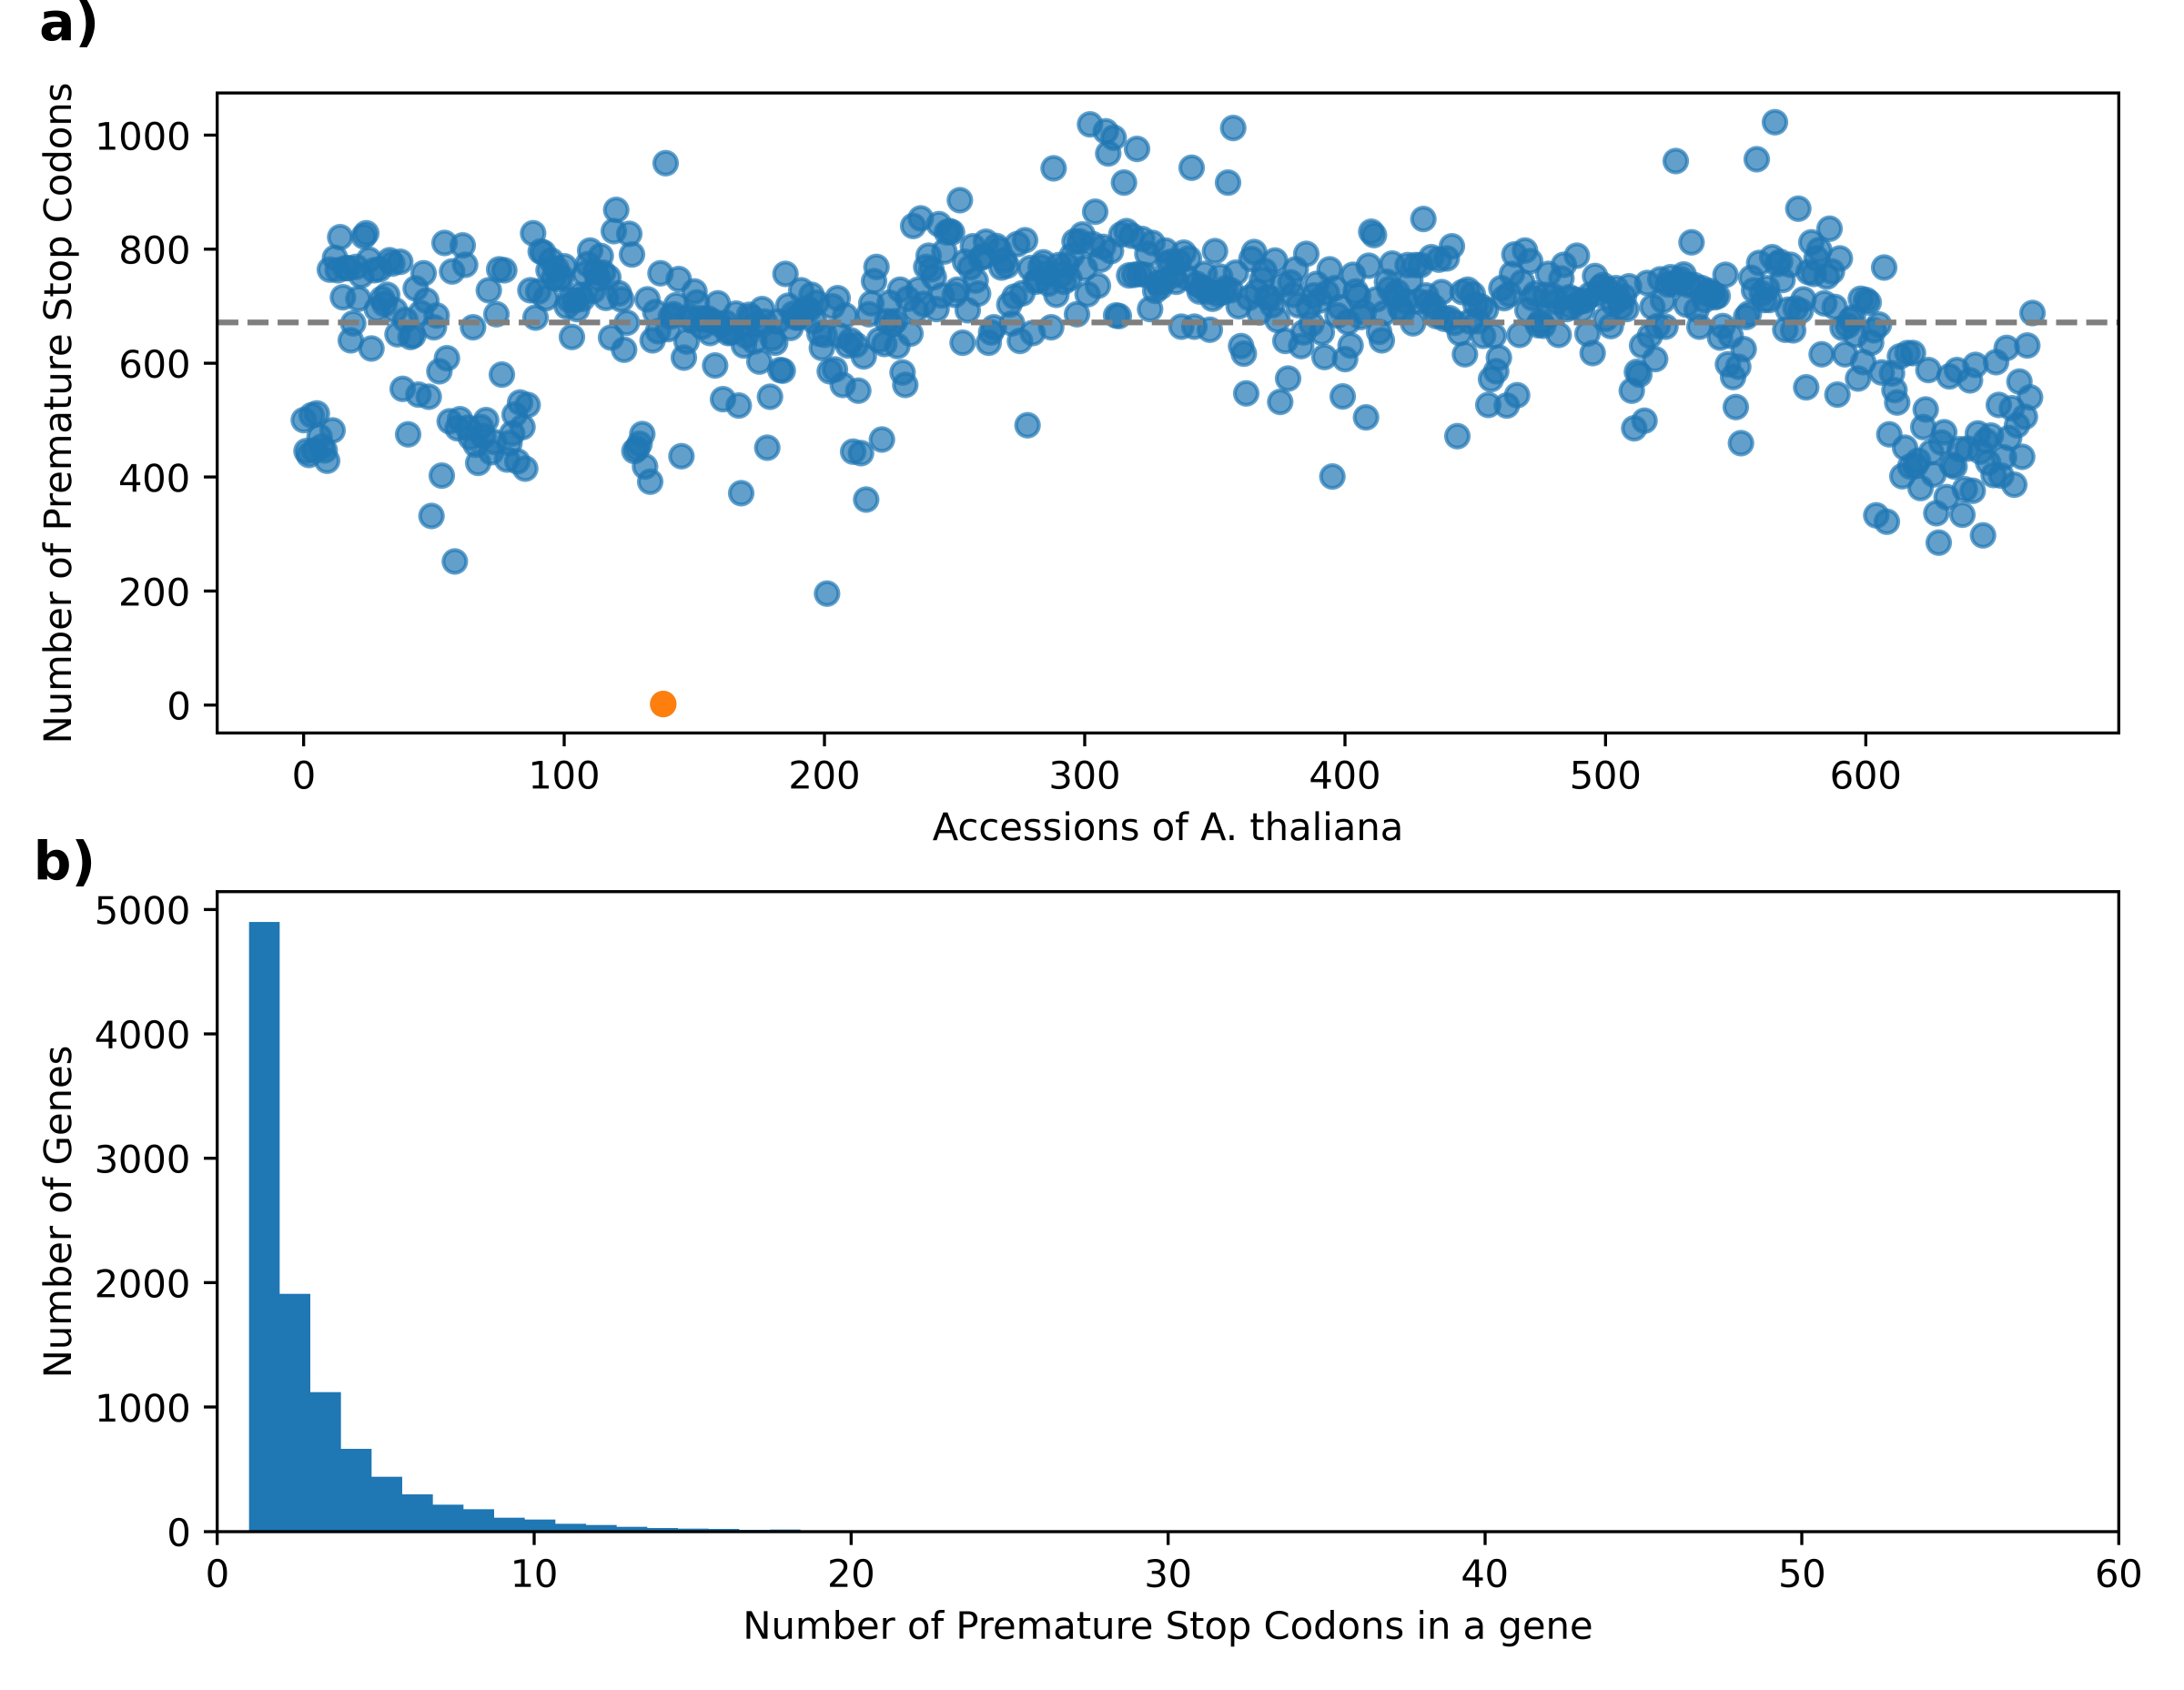
\includegraphics[width=1\textwidth]{images/Distribution_Premature_Stop_Codons.png}
      \caption[Distribution of premature stop codons in the genome from the 665 accessions \textit{A. thaliana} population]{\textbf{Distribution of premature stop codons in the genome from the 665 accessions \textit{A. thaliana} population}\\
      a) Distribution of premature stop codons along the 665 accessions. In each accession many hundreds of premature stop codons exist across the whole coding sequences of the genome. We find an average number of 671 premature stop codons per accession (as indicated in grey). The accession col-0 (138 colored in orange) is an exception since it serves as the reference genome. b) Histogram counting the number of stop codons in a gene. In roughly half of the genes only a single premature stop codon occurs. As one can see the number of genes containing several premature stop codons drops dramatically as a function of this parameter.}
     \label{fig:Distribution_Premature_Stop_Codons_all}
    \end{minipage}
  \end{figure} 

  If we now look at the distribution of premature stop codons in this knock-out genes, we find that roughly half of the genes are knocked out by a single premature stop codon as shown in \autoref{fig:Distribution_Premature_Stop_Codons_all} b). This corresponds to our expectation while we do not expect the alternative.  These other genes contain several premature stop codons. Ranging from 2 to 59 premature stop codons per gene the number of genes containing an increasing number of premature stop codons drops dramatically as a function of this parameter. In the biochemical context two distinct premature stop codons in a single gene of an individual does not seem to make much sense. After the first premature stop codon the translation of the protein stops and the protein is truncated at that point. All following premature stop codons don't have any influence on the protein translation. But this is not the phenomenon we observe in our dataset. The accumulation of premature stop codons in our dataset  is caused from two different phenomena. The first phenomenon which is true for the main part of these gene is triggered by the population structure. In some individuals we observe the first premature stop codons in a particular gene. On the other hand in part of the other individuals, which do not have the first premature stop codon, they include another premature stop codon in a later sequence position. This means that at population scale we do observe several possible premature stop codons in a gene but looking at each individual we see just one premature stop codon for this gene. An exception occurs for a small amount of genes. In these genes we observe an effect of the splicing variants. After the transcription process in eukaryotes the pre-mRNA is build and processed by splicing out the introns and connecting the exons. This means that mutations in the introns does not effect the translation process afterwards. In our analysis we define a gene purely based on the start and the stop of a sequence. We do not consider different splicing forms or intron and exon structures. Therefore we include genes which do have a premature stop codon in an intron or in an exon. 
  
  Considering the occurrence of multiple premature stop codons in a single gene we decided to generate a high confidential dataset with premature stop codons that pass a quality measurement to be sure we work with the ones, which actually influence the protein functionality.
\section{Generation of a high confidential dataset}
As explained in the section before we continue our analysis with the selection of premature stop codons with a high confidential functional dataset. We filter our dataset to be certain that we have functional premature stop stop codons, i.e. we have premature stop codons which do have an influence on protein functionality. We follow two different approaches for generation such a dataset. The first approach is based on the expected difference on gene expression and categorize the premature stop codons in quality classes. The second approach is based on the idea that the remaining length of an mRNA matters for protein functionality. This approach classifies premature stop codons separately and we compare both approaches in the end.  
\subsection{Approach 1: Gene expression differences}
Our first approach is based on the comparison of gene expression differences and thereby categorizing premature stop codons into groups. As explained in \autoref{sec:Methods_Approach_Gene_Expression} we proceed the analysis by some filtering steps. We start with 29029 premature stop codons distributed over the genomes of the 1,135 accessions of \textit{A. thaliana}. After removing all premature stop codons, which are located in newer reported genes or so called pseudogenes, which are just included in the Araport11 annotation, 17046 premature stop codons remain. The reason for this step is explained in the methods \autoref{sec:Methods_Approach_Gene_Expression}.

We classify for each premature stop codon a group of accessions, which includes (knock-out accessions) and which does not include the premature stop codon (wildtype accessions) as described in \autoref{sec:Methods_Approach_Gene_Expression}. Due to the smaller number of accessions for which genomic and transcriptomic data are available we added another filtering step. This removes premature stop codons, which are not included in the 665 accession dataset anymore (see \autoref{sec:Methods_Approach_Gene_Expression}). We end up with 7124 premature stop codons for which we can calculate a t-test quantifing the transcript level changes. 

We classify each premature stop codon into one of three categories. The first category represents unsignificant premature stop codons, which do not show a significant gene expression change between wildtype accessions and knock-out accessions as shown in \autoref{fig:Cathegories}. This can be a matter of similar transcript levels in both groups but could also be a matter of statistical power. If one of the wildtype or knock-out group is very small in proportion to the other the t-test looses its power to determine the level of difference and therefore the p-values returned by the t-test are bigger than the significance threshold. The unsignificant premature stop codons in the first cathegory represent these mutations, where we can't determine the effect on the protein functionality. 

\begin{figure}[tb]
  \centering
  \begin{minipage}[h]{0.9\textwidth}
    \centering
    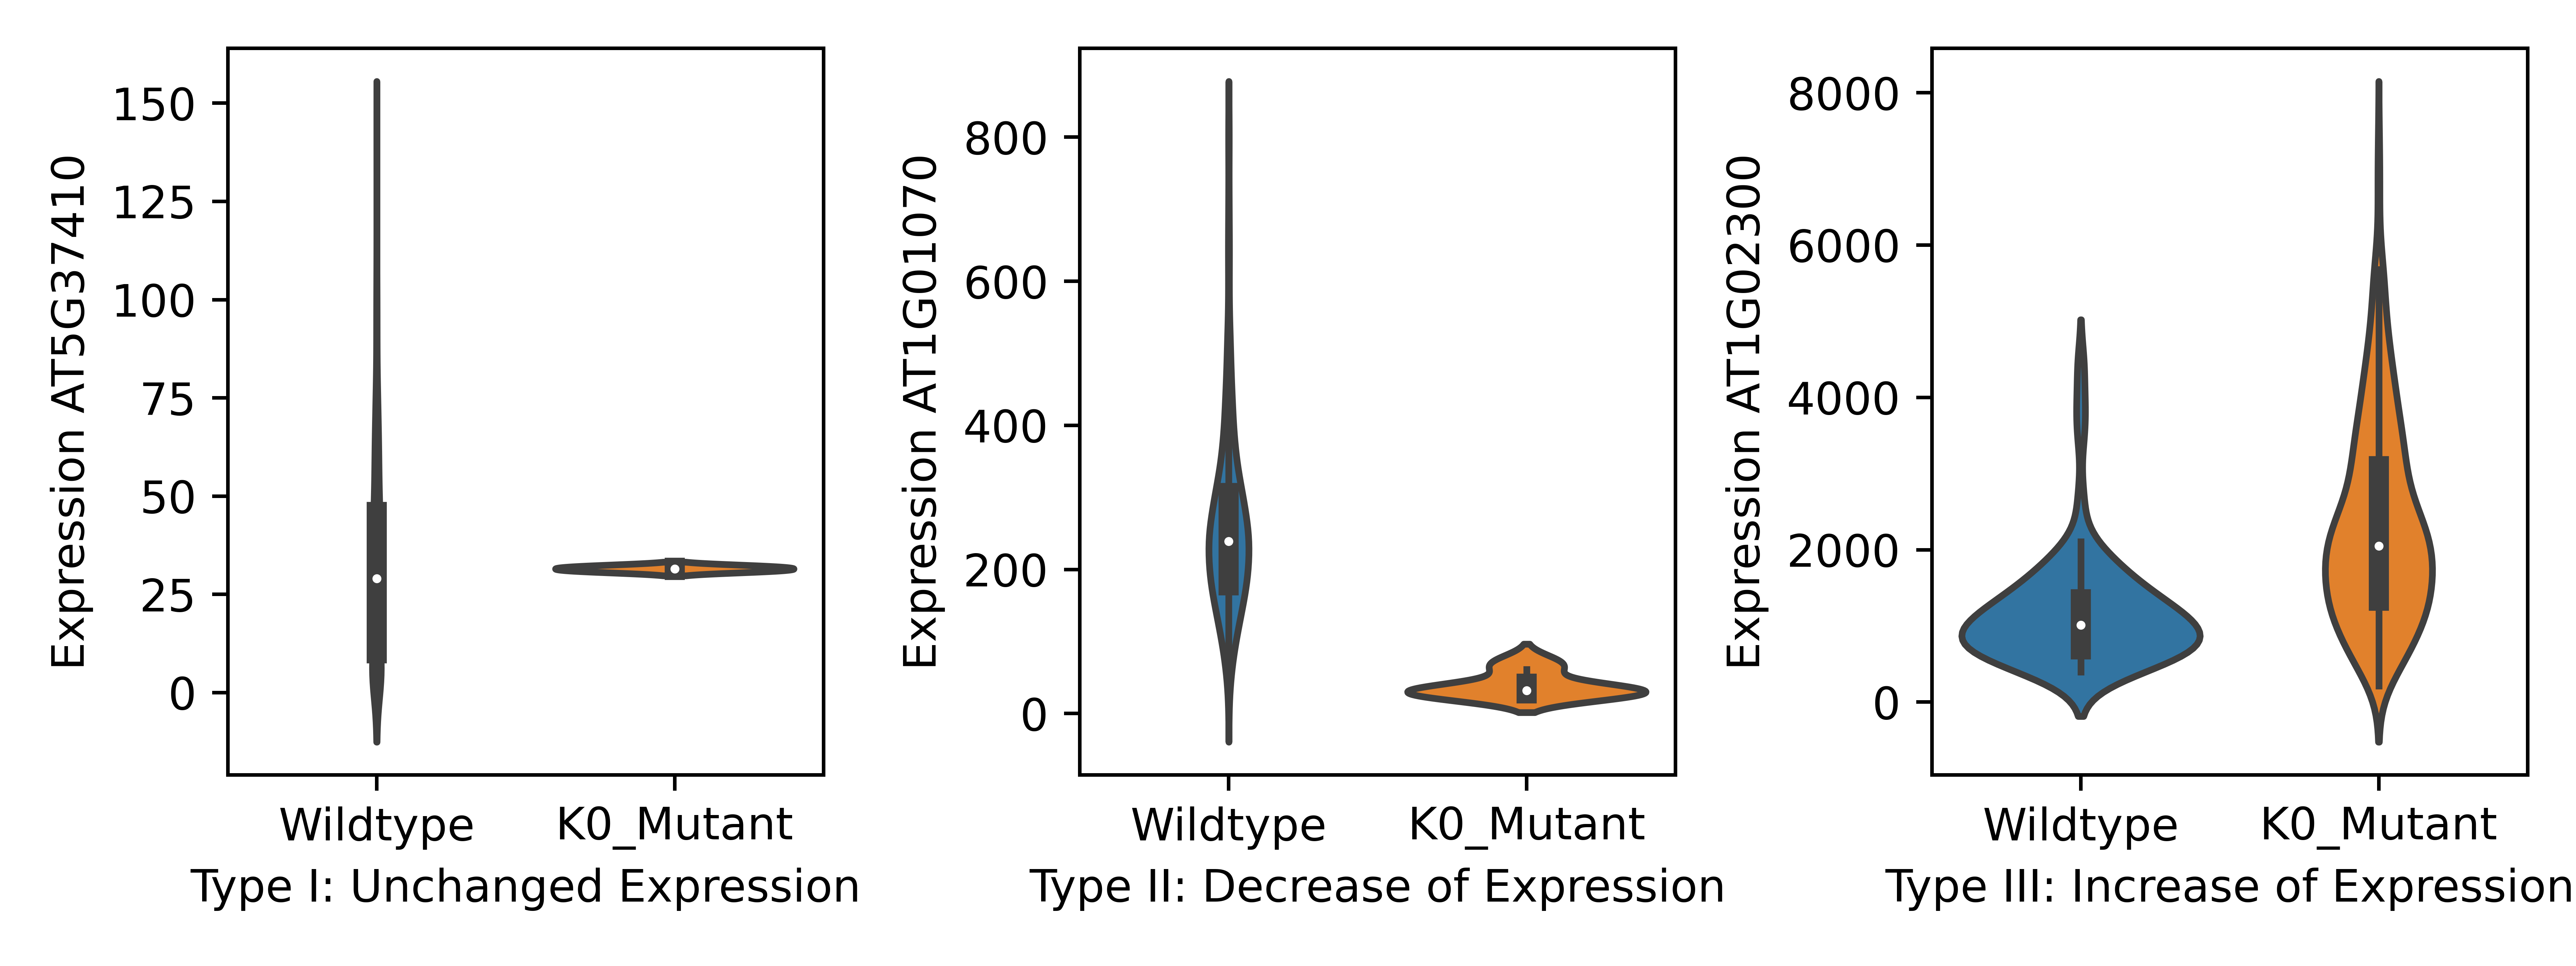
\includegraphics[width=1\textwidth]{images/Cathegories_Premature_Stop_Codons.png}
    \caption[Cathegories of Premature Stop Codons]{\textbf{Examples for each of the three categories of Premature Stop Codons in \textit{A. thaliana}}\\
    (left) Example of the first category representing premature stop codons with an unsignifcant change between the expression level of ATG37410 between wildtype and knock-out accessions. (middle) Example of the second category representing premature stop codons with a decrease of gene expression in knock-out accessions in relation to wildtype accessions in the gene AT1G01070.
    (right) Example of the third category representing premature stop codons with an increase of gene expression in knock-out accessions in AT1G02300.}
   \label{fig:Cathegories}
  \end{minipage}
\end{figure} 

The second category of premature stop codons are those, which decreases the expression of a gene when comparing wildtype and knock-out accessions. An example of this second category can be seen in \autoref{fig:Cathegories}. The decrease of gene expression can be explained by the biochemical process of nonsense-mediated decay (NMD). In this process mRNAs, which contain premature stop codons get eliminated to reduce the amount of loss-of-function variants of that protein (Baker 2004 \cite{Baker2004}). This process allows us to correlate the severity of the premature stop codons to the gene expression level, which we can measure by mRNA sequencing. Applying a p-value threshold of 0.05 to the gene expression decrease filters the number of premature stop codons to 949 as is summarized in \autoref{tab:Categories}. Applying an even stricter p-value threshold that corrects for the multiple testing extracts 247 premature stop codons, which do have a significant decrease and therefore they imply with a high confidence the impact on protein functionality. This dataset is called high confidential dataset and in the following used for further analysis. 

\begin{table}[tb]
  \caption[Three Cathegories of Premature Stop Codons and their related numbers of stop codons of the 665 accession \textit{A. thaliana} dataset]{\textbf{Three Cathegories of Premature Stop Codons and their related numbers of stop codons of the 665 accession \textit{A. thaliana} dataset}\\
  The numbers of premature stop codons in each of the three categories is calculated based on a statistical t-test as explained in \autoref{sec:Methods_Approach_Gene_Expression}. The premature stop codons are classified using two different p-value thresholds, the first the common 0.05 threshold and the second corrected for multiple testing.} 
  \label{tab:Categories}
  \centering
  \begin{tabular}{|l|l|l|l|}
  \hline
  \begin{tabular}[c]{@{}l@{}} \textbf{p-value} \\ \textbf{threshold} \end{tabular} & \begin{tabular}[c]{@{}l@{}} \textbf{Type I:} \\ \textbf{Unchanged Expression} \end{tabular} & \begin{tabular}[c]{@{}l@{}} \textbf{Type II:}\\ \textbf{Decrease of Expression} \end{tabular} & \begin{tabular}[c]{@{}l@{}}\textbf{Type III:} \\ \textbf{Increase of Expression} \end{tabular} \\ \hline
  0.05 & 5433 & 949 & 742 \\ \hline
  bonferroni & 6608 & 247 & 269 \\ \hline
  \end{tabular}
  \end{table}                  

  The last category of premature stop codons are those, which show an unexpected pattern of gene expression change. Instead of decreasing the gene expression with nonsense-mediated decay they actually increase their gene expression significantly as shown in \autoref{fig:Cathegories}. Applying the commonly used p-value threshold of 0.05 we group 742 premature stop codons together in this category. Even with the stricter bonferroni threshold we found 269 premature stop codons, which significantly increase the gene expression in knock-out accessions. This group of premature stop codons is definitely an unexpected finding. At the moment we do not have an explanation why these premature stop codons show this expression change. Although they belong to an interesting group, which could help to explain new biological insights, this class of premature stops is excluded from our further analysis. 
  
  \subsection{Approach 2: Remaining length of the protein}
  A separate approach to generate a high confidential dataset of premature stop codons is based on the length of the remaining protein. If a stop codon emerges into a coding sequence the corresponding protein is truncated at that point. Dependent on the remaining length of the protein the functionality of a protein should be affected. Wee calculate the remaining length for all 29029 premature stop codons in a relative measure and observe a u-shaped distribution as shown in \autoref{fig:Length}. 

  \begin{figure}[tb]
    \centering
    \begin{minipage}[h]{0.9\textwidth}
      \centering
      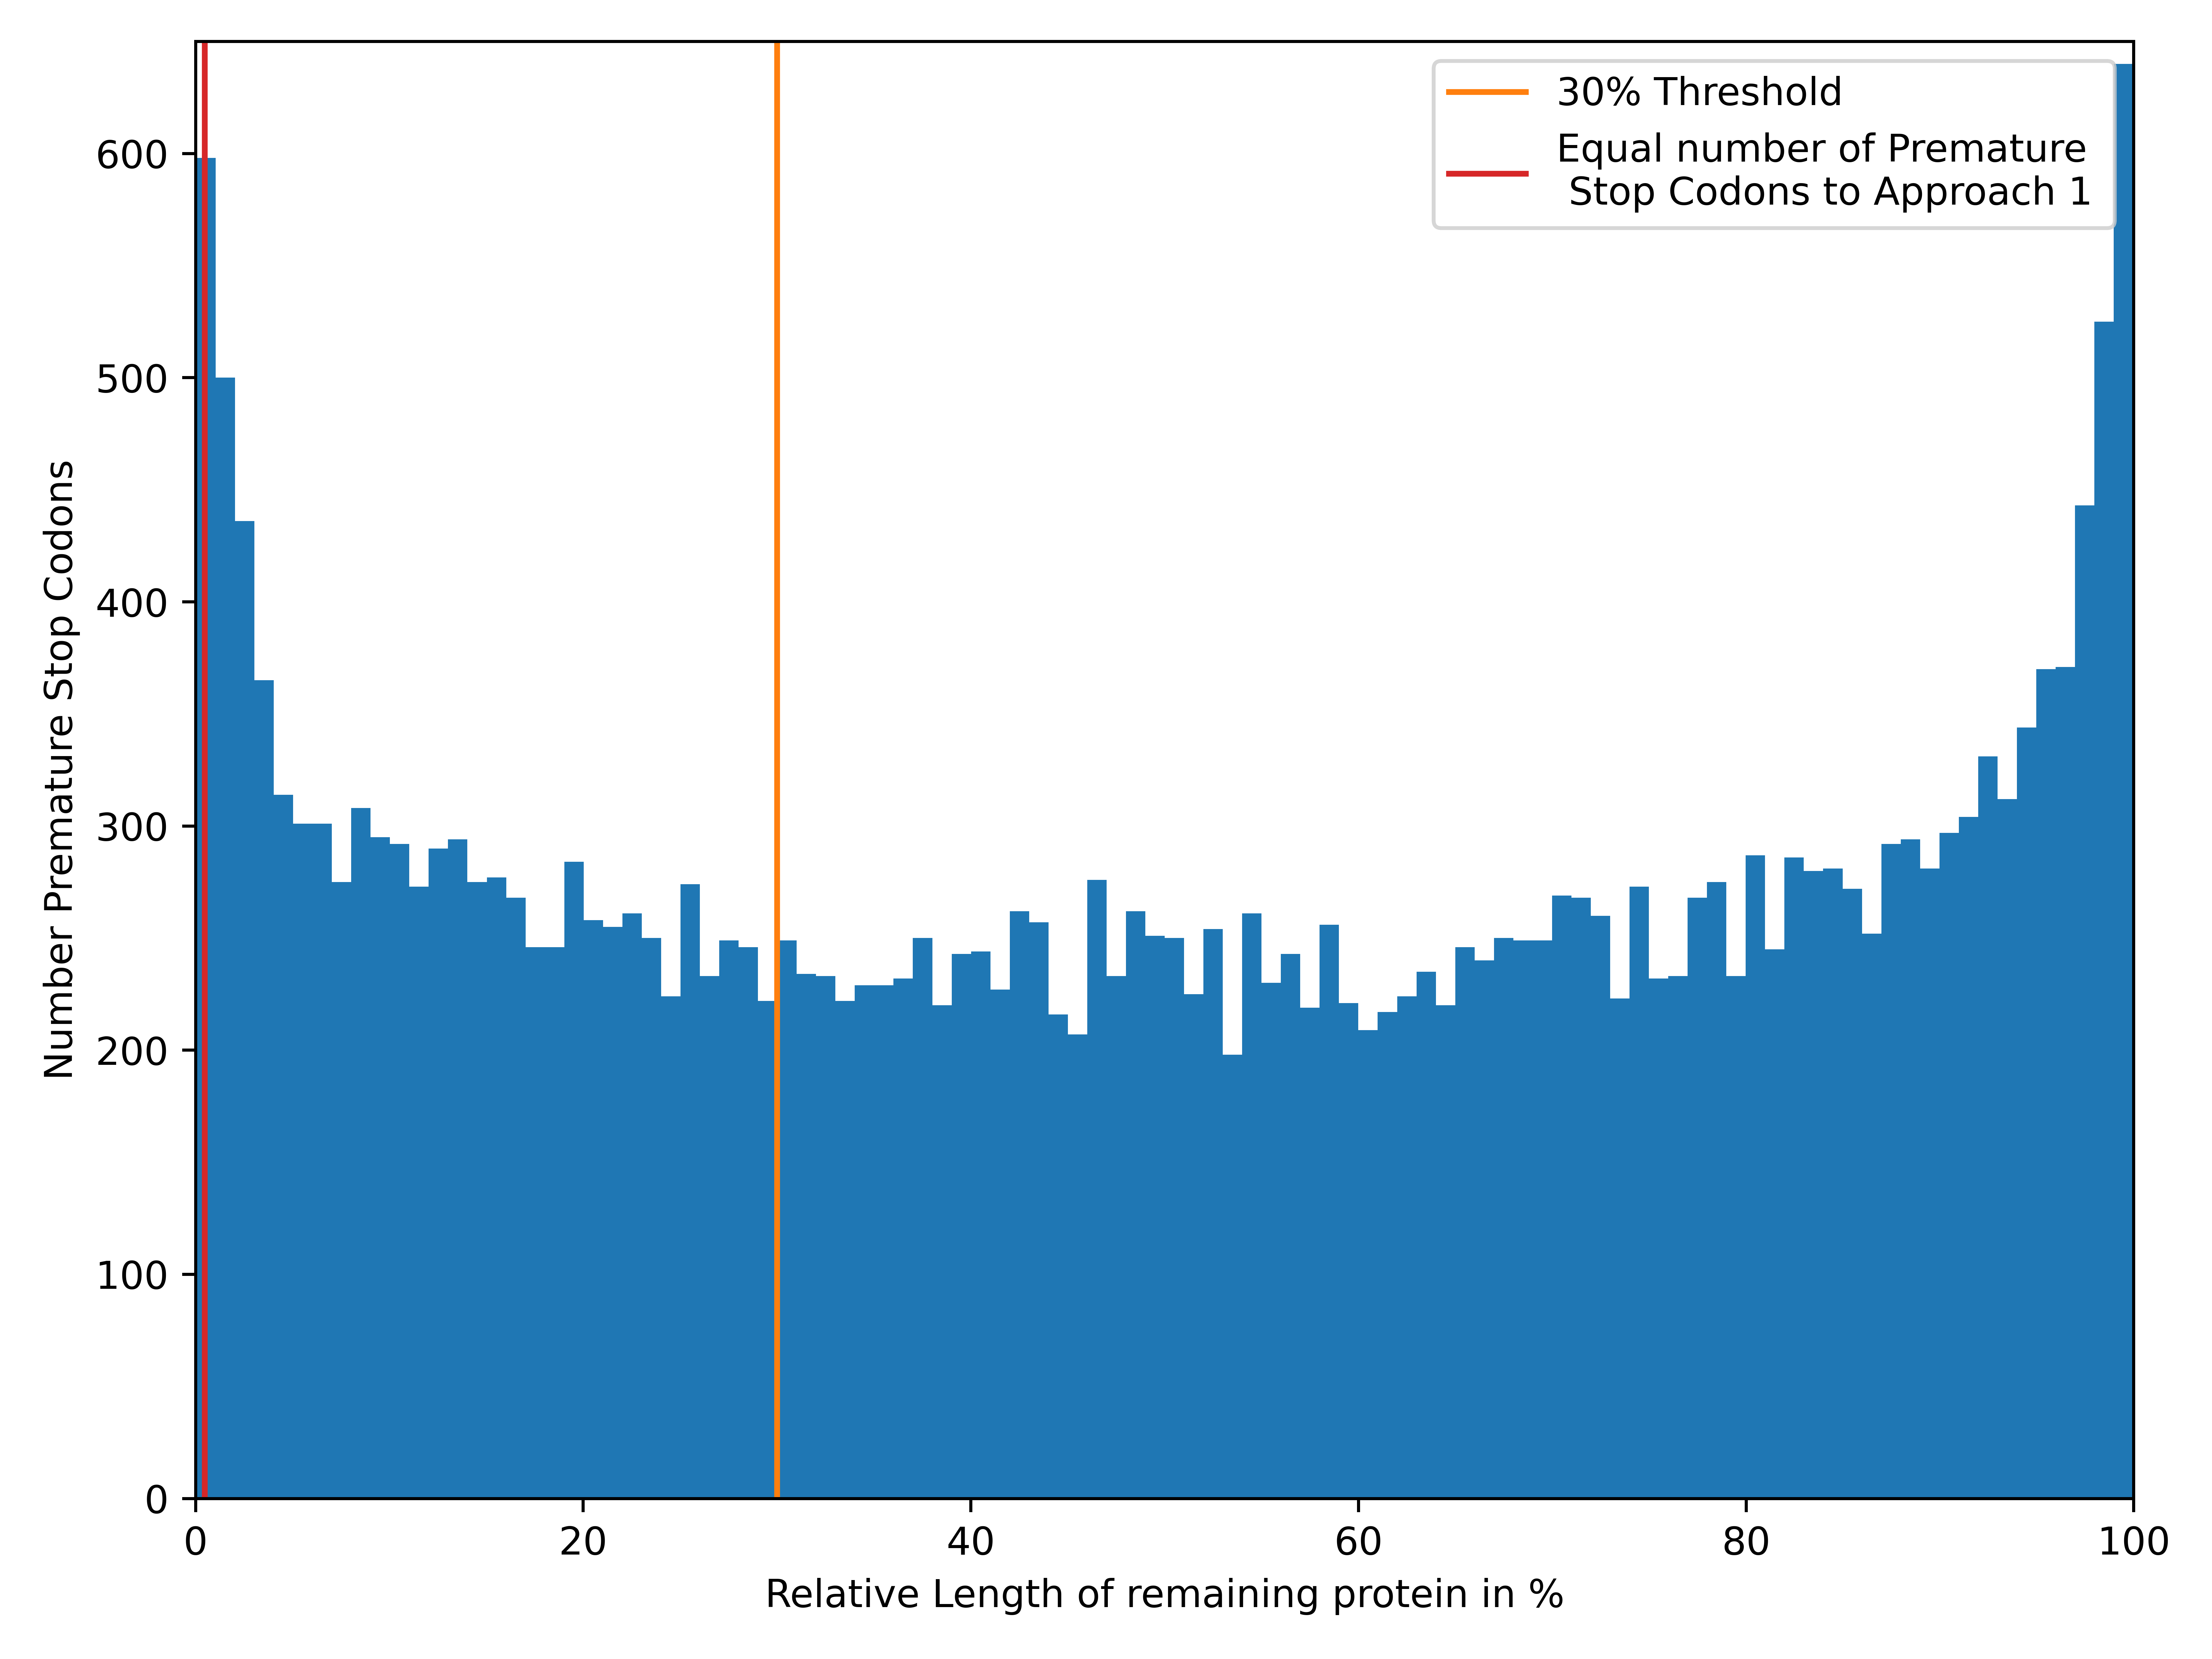
\includegraphics[width=1\textwidth]{images/Remaining_Length.png}
      \caption[Distribution of relative protein lengths after premature stop codon emergence.]{\textbf{Distribution of relative protein lengths after premature stop codon emergence in the 29029 premature stop codons of 1,135 accession of \textit{A. thaliana}}\\
      Visualized are the calculated relative lengths based on the fraction of the length after an emergence of a premature stop codon and the original length of the protein. The 29029 premature stop codons form a U-shaped distribution by accumulating in very small remaining lengths and in the opposite direction, where nearly full remaining lengths accumulate. The orange threshold line separates the left subset of premature stop codons which have a smaller than \SI{30}{\percent} remaining length. The red threshold line shows a number of 247 genes, which is equal to the size of the high confident dataset of approach 1 generated based on significant decreased gene expression.}
     \label{fig:Length}
    \end{minipage}
  \end{figure} 
  
This distribution demonstrates the evolutionary selection force that drives premature stop codon accumulation in the genetic pool. Premature stop codons that do not truncate the original protein by more than \SI{20}{\percent} accumulate in the 1,135 population of \textit{A. thaliana}. In this group the effect on the protein functionality is less severe compared to the other premature stop codons since a nearly complete protein is translated. 

Decreasing this relative remaining length decreases also the observed premature stop codons as the expected severity increases. Unexpectedly we find an accumulation of premature stop codons, which provoke a very short remaining protein. We observe 18718 premature stop codons resulting in proteins with \SI{30}{\percent} remaining length. Selecting a subset equal in size compared to the previous generated high confident dataset from approach 1 (247) we select just premature stop codons, which provoke a remaining length of the protein of \SI{0.47}{\percent}. 

Having obtained the distribution of relative lengths initiated by premature stop codons lets us hypothesize on the selection force on these population of 1,135 accessions of \textit{A. thaliana}. Premature stop codons which appear at the end of a protein, truncate the protein but may not always lead to a loss-of-function. These premature stop codons accumulate in the genetic pool of a population since they seem not to be under a strong natural selection. On the other hand proteins that are truncated in a middle region between 20 to 80 percent of the original length provoke a loss-of-function in the protein. Therefore natural selection acts on them and they get reduced in the genetic pool. Quite different acts the natural selection on very short remaining proteins. By emergence of a premature stop codon in the first \SI{20}{\percent} of the protein the protein looses its function. But instead of reducing these variants of genes from the genetic pool natural selection stabilize them since we see a increase of them in our dataset. We hypothesize that this increase is caused by effecting the underlying gene-regulatory network since it seems that instead of destabilizing it, adding new ways of adaptation can be positive for different environmental conditions. This may allow the individual to gain a profit of such a premature stop codon and therefore natural selection accumulates these variants in the genetic reservoir of a population.

\subsection{Comparing the two approaches}
In the following we are interested in comparing the subsets of premature stop codons, that we extracted with our two approaches. First we compare equal amount of premature stop codons in two subsets. Therefore we look at the bonferroni significant premature stop codons, which decrease their gene expression and took the equal amount of premature stop codons with the shortest length. Each of the subsets consists of 247 premature stop codons but just 3 premature stop codons are contained in both subsets, which can be seen in the venn-diagram of \autoref{fig:Venn_Diagram} a). This unexpectedly small overlap of the two subsets could be linked to the high amount (600) of premature stop codons, which provoke less than \SI{1}{\percent} of the original protein. Since we build the subset based on the remaining length we just took the first 247 premature stop codons and invoke a threshold at a remaining length of \SI{0.47}{\percent}. We nevertheless want to know if the significant decrease in gene expression correlates with the relative length of the resulting protein. 

\begin{figure}[h!]
  \centering
  \begin{minipage}[h]{0.9\textwidth}
    \centering
    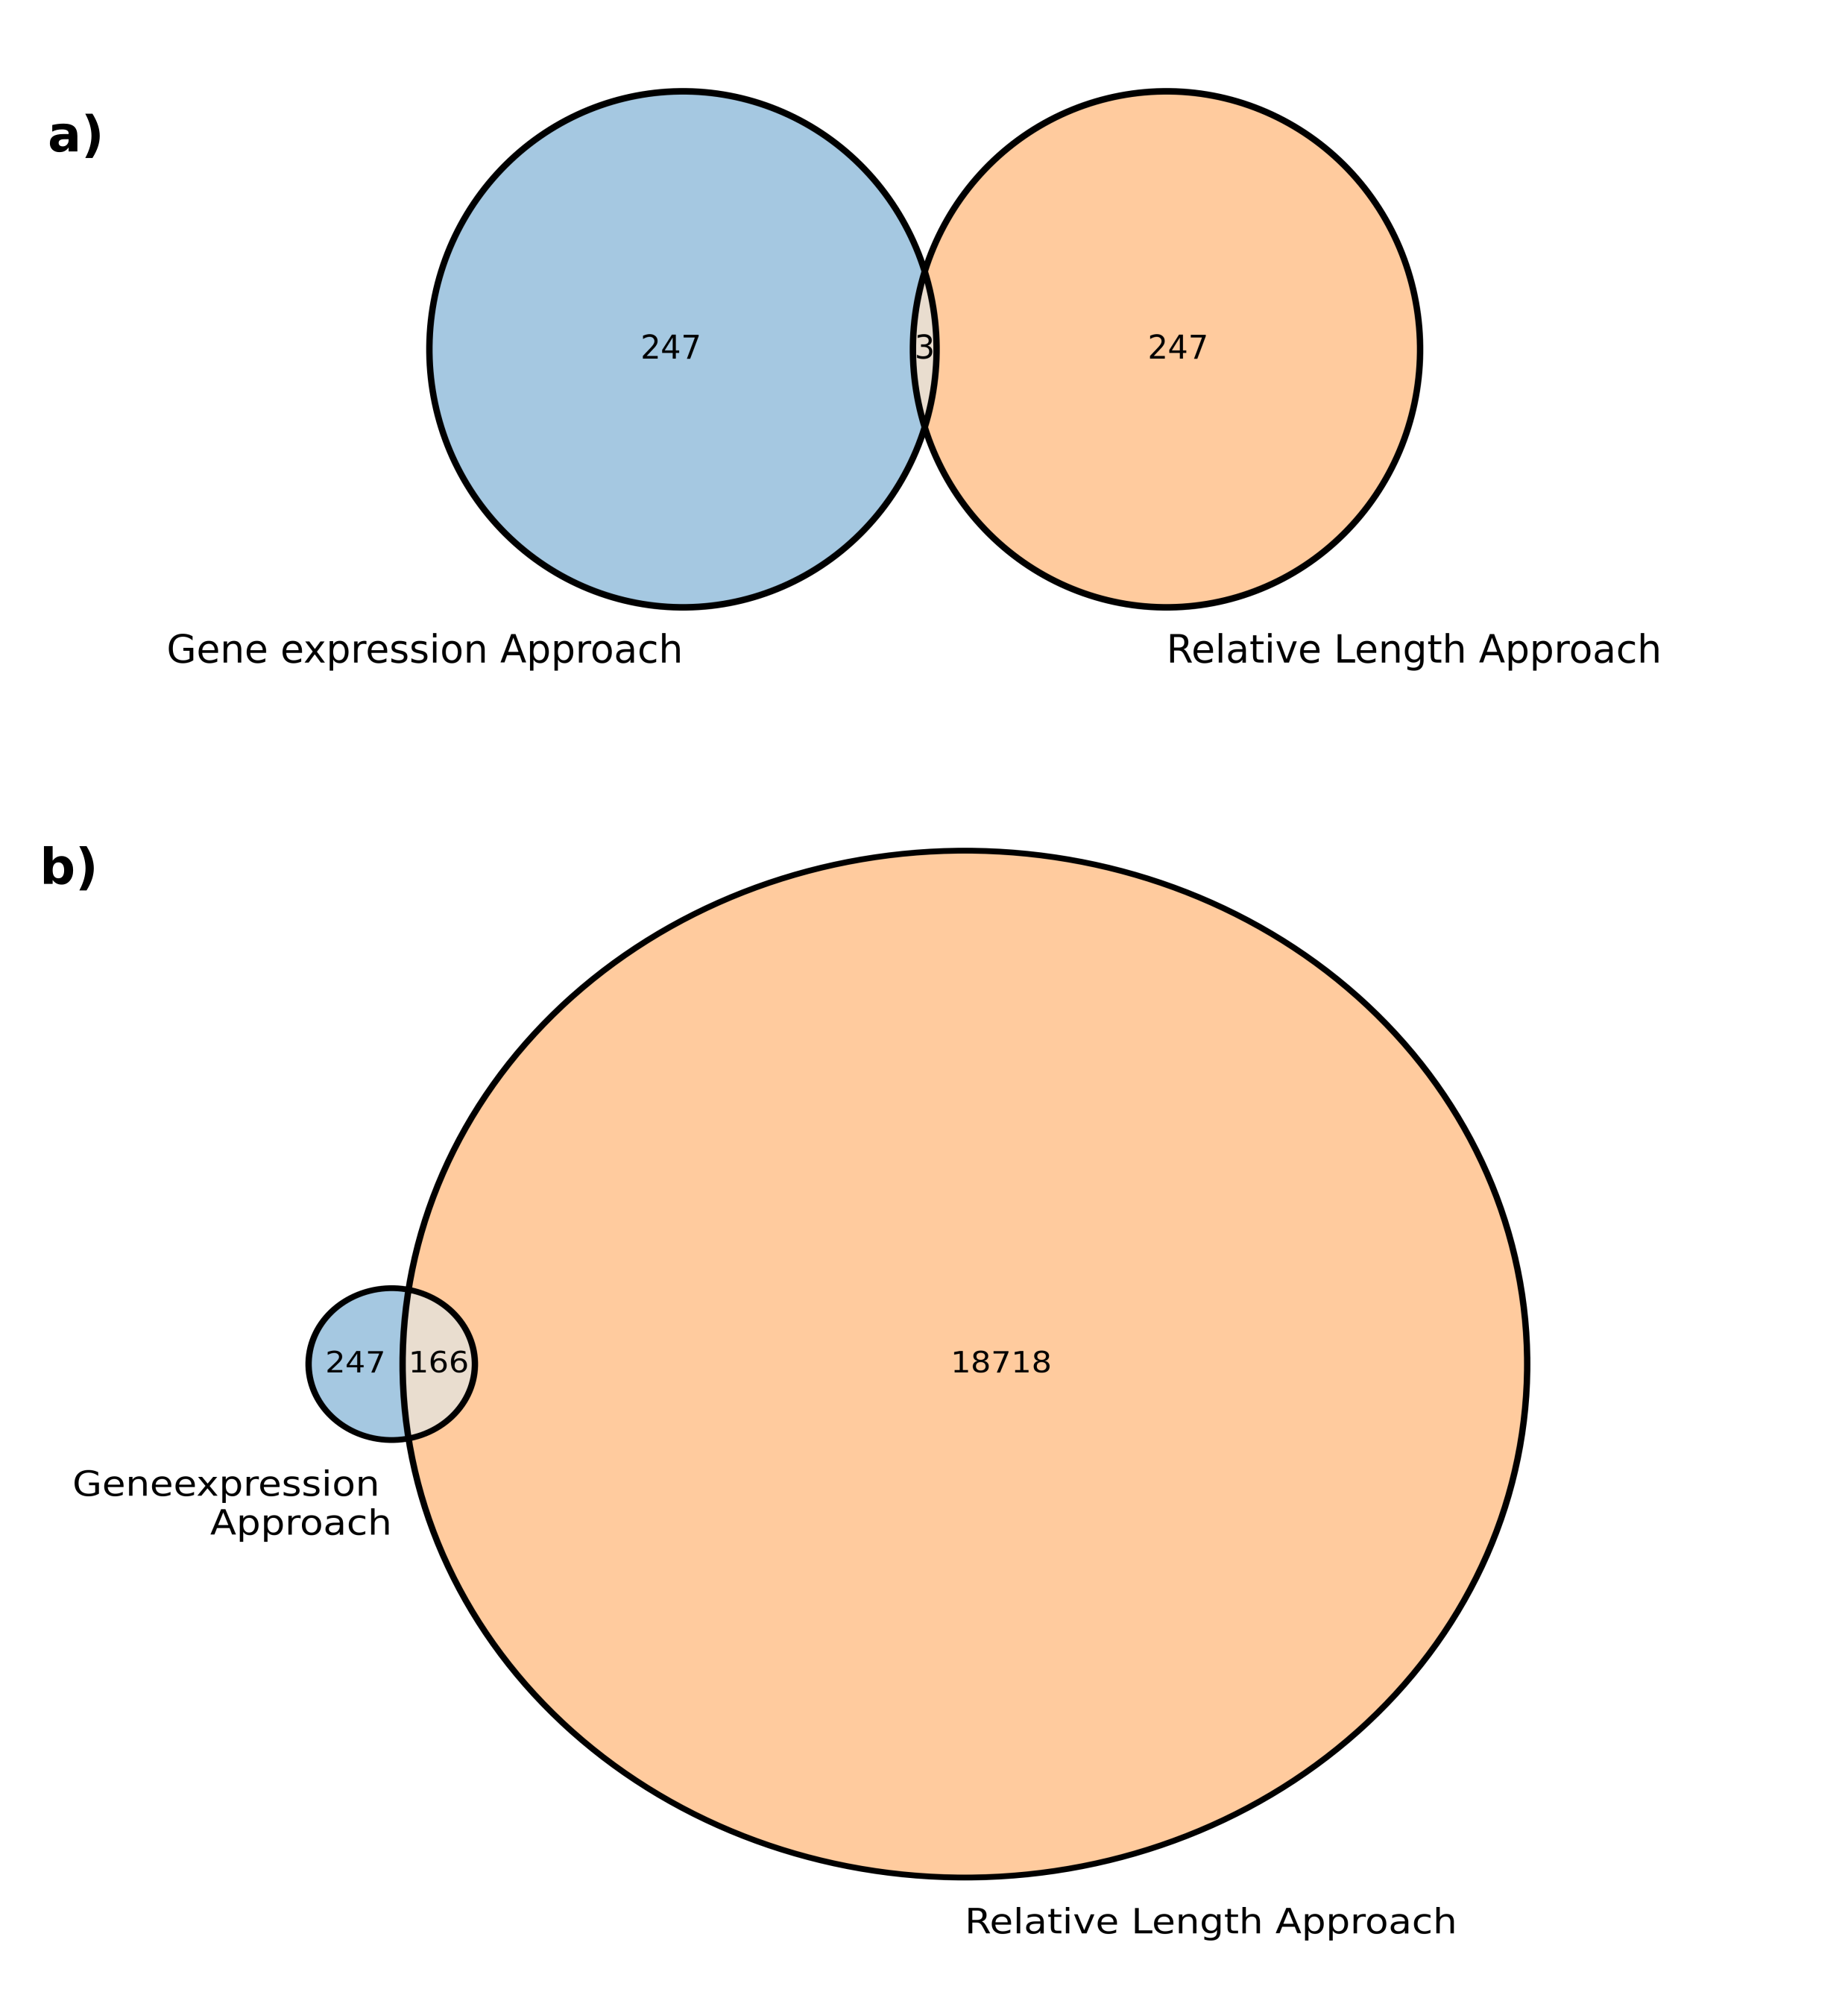
\includegraphics[width=1\textwidth]{images/Venn_Diagramms.png}
    \caption[Venn Diagrams showing the similarities of selected premature stop codons  of the two subsets created with the two previous approaches]{\textbf{Venn Diagrams showing the similarities of the two subsets of selected premature stop codons  created with the two previous approaches}\\
    a) The bonferroni significant gene expression decreased premature stop codons of approach 1 contain 3 identical premature stop codons when the relative length subset is cutted with AN equal amount of premature stop codons (247). b)
    The subset of premature stop codons, which provoke \SI{30}{\percent} left from the original protein, containS 166 premature stop codons that are also included into the bonferroni significant decreased gene expression dataset.}
    
   \label{fig:Venn_Diagram}
  \end{minipage}
\end{figure} 

To answer this question we check the second subset of the relative length approach which contains all premature stop codons, that provoke less than \SI{30}{\percent} of the original protein. This subset consists of 18,718 premature stop codons and it has an overlap with the subset of the gene expression approach of 166 premature stop codons. These numbers are illustrated in \autoref{fig:Venn_Diagram} b). This means that more than half of the premature stop codons which are included into the gene expression subset are also included into the subset of the relative length approach. On the other hand half of the premature stop codons of the subset of the first approach are not included. Therefore we can see that the relative length of the remaining protein does matter for reducing the gene expression of this gene but it definitely is dependent on other factors. The relative length alone does not effect the gene expression entirely. 

Based on this results we decided to work further with the subset of premature stop codons which decrease their gene expression in the knock-out accessions with bonferroni significance. 

\section{Interactions between premature stop codons}
Building on our selected high confidential dataset of premature stop codons, which includes all premature stop codons (see \autoref{sec:Methods_Approach_Gene_Expression}) with bonferroni corrected significant gene expression decrease, we want to study further how premature stop codons interact in gene regulatory networks. To accomplish this we combine single premature stop codons to a more compressed level of gene-based premature stop codons. This means we compress the dataset of 247 single premature stop codons into 216 gene based stop codons by following the described process in \autoref{sec:Methods_Approach_Gene_Expression}.

From this compressed list of gene-based premature stop codons we build pairs of interactions with all possible combinations of premature stop codon pairs. For each of these interaction pairs we calculate the cooccurrence of both premature stop codons and perform a hypergeometric test as explained in the \autoref{sec:Methods_Coocurrence}. By applying the commonly used p-value threshold of 0.05 we can identify 19208 premature stop codons that show an over-coocurrence. 
An over-coocurrence means, that for each of these interaction pairs we observe the two premature stop codons existing together in a genome of an accession more often than we would expect them for a random distribution. We also observe 134 premature stop pairs with an under-cooccurrence, which represent accessions, which do contain less often than expected the two premature stop codons together. The numbers of premature stop pairs are summarized in \autoref{tab:Coocurrence}. 
\begin{table}[tb]
  \caption[Coocurrence in pairs of premature stop codons]{\textbf{Coocurrence in pairs of premature stop codons}\\
  From the gene-based high-confident premature stop codons are pairs of premature stop codons analysed, and by performing a hypergeometric test the coocurrence of each pair is evaluated. Applying a common used p-value of 0.05. 19208 pairs of premature stop codons are more linked together than can be expected from the distribution in the population of 665 accessioons of \textit{A. thaliana}. And 134 pairs are occurring less often together than one would expect. If the stricter bonferroni corrected threshold is applied we remain with 1128 premature stop codons which occur more often together than it can be expected by the population distribution. Moreover no premature stop codons come together less often than expected. }
  \label{tab:Coocurrence}
  \centering
  \begin{tabular}{|l|l|l|}
  \hline
  \textbf{p-value threshold} & \textbf{over-cooccurrence}  &  \textbf{under-cooccurrence}  \\ \hline
  0.05 & 19208 &  134 \\ \hline
  bonferroni-corrected & 1128 &  - \\ \hline
  \end{tabular}
  \end{table}

To exclude the increasing amount of false positives, which we observe due to multiple tests on our dataset, we need to correct our p-value threshold to the bonferroni corrected threshold. The number of premature stop pairs, which show a bonferroni significant cooccurrence decreases to 1128 pairs of premature stops, while correcting our p-value threshold removes all under-cooccurrence pairs. 

These results are stunning in light of their biological interpretation. Since we selected a high-confidential dataset by correlating this to an establishment of a loss-of-function variant we found unexpected interaction pairs. These interactions occur more often than can be expected by chance. This means that an accession, which does have one premature stop codon, experience a selection force to gain also the belonging second premature stop codon. In the evolutionary context this means, that such an accession gains a fitness advantage since it can adapt to the environmental factors better than others. such a selection on cooccurring premature stop codons should be prevented through evolutionary selection otherwise and we should not have found significant over-coocurrence in the natural variation dataset of \textit{A. thaliana}. We can further see for the under-coocurring pairs of premature stop codons, that our hypothesis, that premature stop codons lead to a stabilization of the surrounding gene regulatory network are not observable in our dataset. On the opposite we find, that these coocurring premature stop codon pairs effect the gene regulatory network in a way that the gain of the first premature stop codons influences the gene regulatory network through a knock-out of this part of the pathway. But instead of stabilizing the surrounding pathways to maintain as much of the original function as possible, a second premature stop codon is preferred to even stronger influence the gene regulatory pathways.
\section{Summary of the premature stop codon analysis}
In the above sections we presented our analysis of the distribution and interaction of premature stop codons. In the following and with the illustration of the workflow in \autoref{fig:Numbers_Workflow} we want to summarize our observations. 

\begin{figure}[h!]
  \centering
  \begin{minipage}[h]{0.9\textwidth}
    \centering
    \includegraphics[width=1.0\textwidth]{images/Numbers_Workflow.png}
    \caption[Overview and summary of the analysis of premature stop codons]{\textbf{Overview and summary of the analysis of premature stop codons}\\
    Our workflow is presented in a schematic figure. All numerical results are included for both approaches to have a quick summary of the actual numbers. The workflow begins with the separation into two approaches to generate a high-confidential dataset. Since the second approach was not carried forward its path ends with the generation of its high-confidential dataset. The other approach based on gene-expression changes was carried further and interactions between pairs of premature stop codons are obtained which lead to the detection of 1128 over coocurrence interactions between gene-based premature stop codon pairs. 
    }
   \label{fig:Numbers_Workflow}
  \end{minipage}
\end{figure} 

We started with the distribution of 29029 premature stop codons and continued by generating a high confidential dataset. To generate this reduced dataset we followed to separate approaches. The first being based on the gene expression differences and the second based on the remaining protein length. The gene expression approach concluded with the generation of a high confidential dataset including 247 premature stop codons with a decreased gene expression between wildtype and knock-out accessions. The second approach, calculating the remaining protein length and subsetting this dataset based on two different thresholds was not carried on and ended in the comparison of this dataset to the first approach. The high confidential dataset including 247 premature stop codons was than compressed into a gene-based list of 216 premature stop codons. Their interaction pairs were studied by a hypergeometric test. These statistical tests resulted in the identification of 1128 over-coocurring premature stop codons. All of these numbers as well as the results presented in the sections above are summarized in \autoref{fig:Numbers_Workflow}. 

\section{Control with synonymous mutations}
\label{sec:Results_Control}
It is intriguing to use the high numbers of premature stop codons, which are linked into pairs as a basis for the study of gene-regulatory networks. In order to quantify how large these numbers are compared to other mutation classes we want to establish a control group and we use synonymous mutations for this purpose since they do not effect protein functionality and therefore have no effect on fitness selection. Comparing synonymous mutations to the premature stop codons we have the possibility to differentiate the effect of natural selection and the background noise distribution.

To accomplish this, we built a control dataset with an equal amount of included gene-based synonymous mutations (216) and select them such that their allele frequency exactly matches the observed allele frequency of premature stop codons. The observed allele frequency is shown in \autoref{fig:Allele_Frequency}. We observe a relatively low allele frequency for most of the included premature stop codons. By increasing the allele frequency the number of premature stop codons drops. Furthermore the distribution is not continuous, i.e. we do not observe premature stop codons for all allele frequencies but rather observe discrete allele frequencies.

\begin{figure}[tb]
  \centering
  \begin{minipage}[h]{0.9\textwidth}
    \centering
    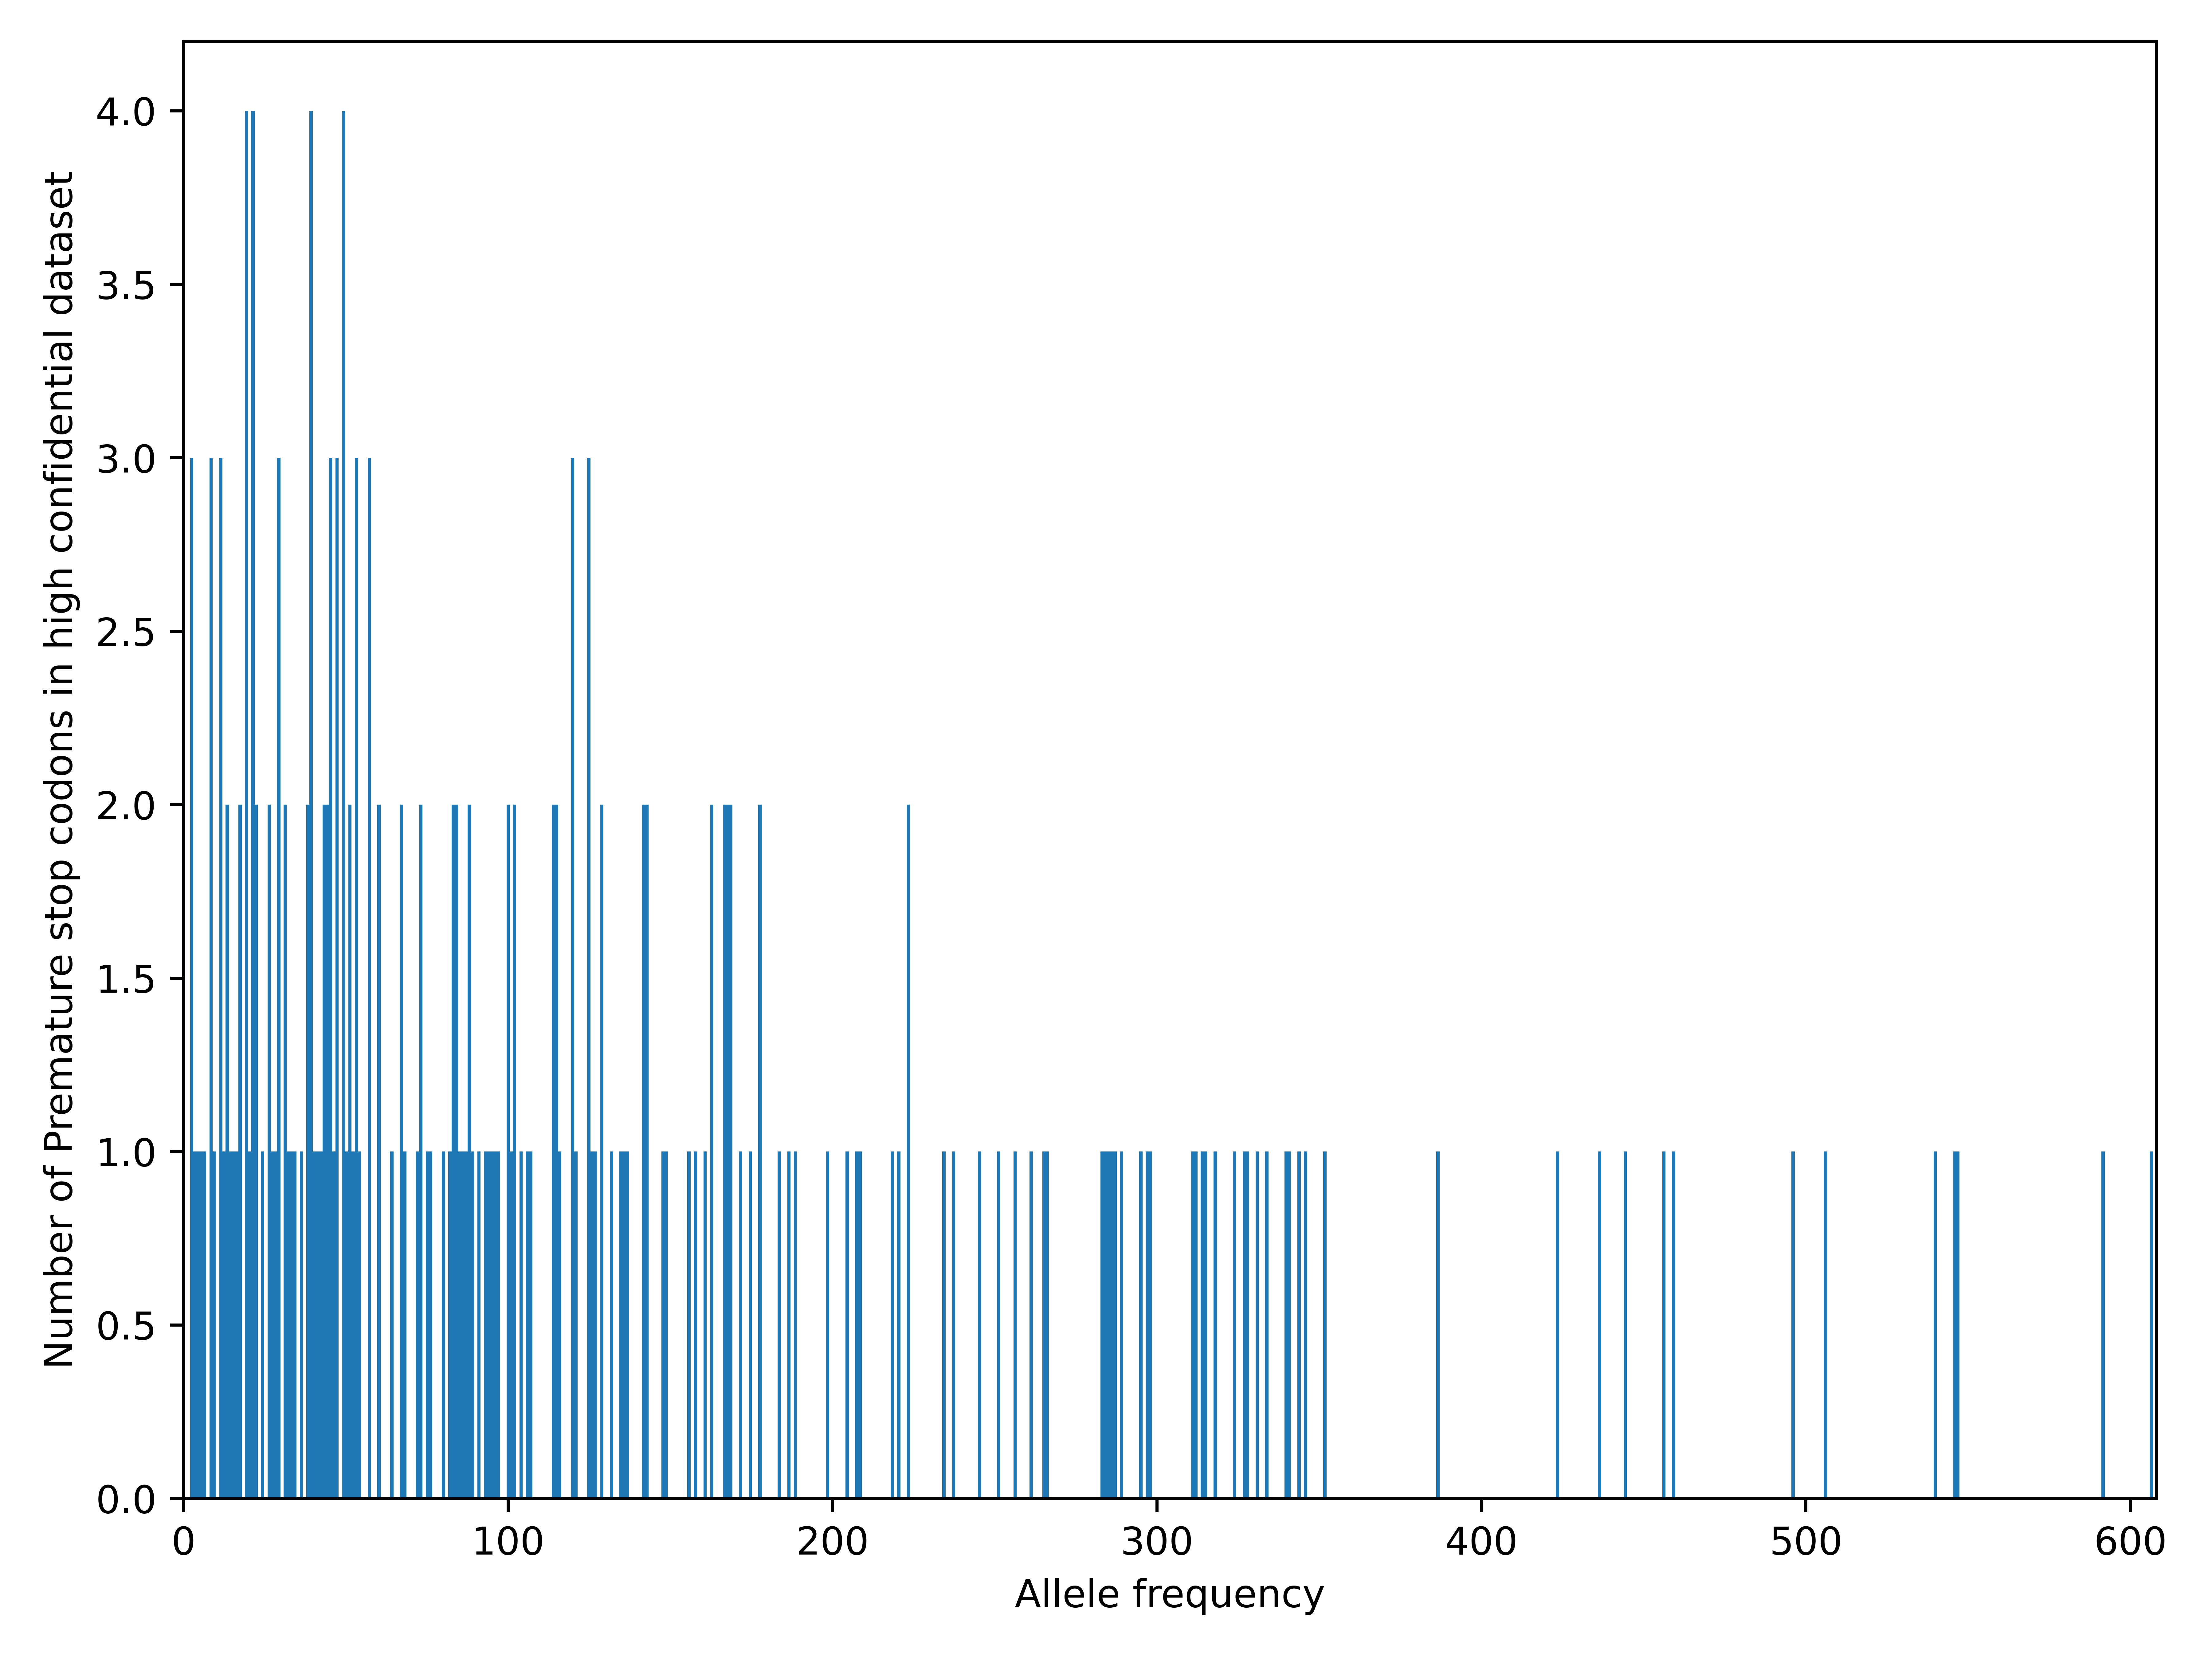
\includegraphics[width=1.0\textwidth]{images/Allele_Frequency.png}
    \caption[Distribution of allele frequency of premature stop codons in the high confidential dataset]{\textbf{Distribution of allele frequency of premature stop codons in the high confidential dataset}\\
    We see the highest amount of premature stop codons with small allele frequencies. The amount of premature stop codons observed in the high confidential dataset drops with the increase of the allele frequency. This distribution of allele frequencies of premature stop codons should be matched by our control dataset with synonymous mutations.
    }
   \label{fig:Allele_Frequency}
  \end{minipage}
\end{figure} 

For the control group, we investigate the coocurrence of synonymous mutations by following the same protocol employed previously for the analysis of premature stop codons. For this we need to match the distribution of allele frequencies as best as possible to the premature stop allele frequency since this allows us to compare the groups. The dataset of 1,135 accessions of \textit{A. thaliana} contains 772,060 synonymous SNPs. This dataset needs to be filtered into the smaller dataset of 665 accessions of \textit{A. thaliana} to adjust the statistical power to the premature stop dataset. We then calculate all allele frequencies of these synonymous SNPs and generate a control dataset by selecting the ones with the right allele frequency in a randomized way. 

Preliminary results of this method show a significantly smaller amount of cooccurring synonymous SNPs, which would confirm the observation of premature stop codons occurring more often in interaction pairs  and even strengthen our biological explanation. Since these allele frequency calculations take a lot of computational resources they were not finished by the time this thesis is written. The exact numbers of this control calculation will have to be evaluated in a later step. 
\newpage
% !TeX root = main.tex
\chapter{Discussion}
Our analysis of the premature stop codons in the 1,135 \textit{A. thaliana} population gives new insights into the effect of natural selection on them. We find premature stop codons distributed all over the 665 accessions of \textit{A. thaliana}. Remarkably not just a few but many hundreds of premature stop codon mutation occur for each accession.  Moreover these are distributed in the population at different positions and even if they emerged in the same gene, different position are observed in the population of \textit{A. thaliana}. 

We analyse the gene expression level of premature stop codons and find three categories. The category in which premature stop codons influence an increase of gene expression in the knock-out accessions are especially interesting for further analysis and so far do not have a biological interpretation. We further gained interesting insights into the distribution of premature stop codons in genes relative to their insertion site and found an accumulation of premature stop codons at the corners for very short and nearly complete remaining proteins. We identify a strong natural selection influencing the premature stop codon in the middle region, where medium remaining proteins result. Our analysis for the comparison of the protein length and mRNA expression based analysis shows, that the gene expression decrease is not entirely correlated to the length of the resulting protein. Even by considering proteins, which just remain with \SI{30}{\percent} of their original length we find genes with a decrease in gene expression, which need to have another influence factor. 

Our analysis of interactions between premature stop codons shows that previous hypothesis of the single occurrence of premature stop codons can not be confirmed in our dataset. We identify pairs of premature stop codons which significantly are linked together on a population scale and hypothesize from these finding a mechanism. This mechanism results in adaptation to an environment by gaining premature stop codons even more by gaining pairs of premature stop codons which positively force the generation of new gene regulatory networks by preventing the functionality of the former ones.  

Already in 2012 MacArthur et al. \cite{macarthur2012} showed, that an average human carries about 100 loss-of-function variants in his genome, without building severe disorders. These results match with our findings of the observed distribution of premature stop codon in \textit{A. thaliana} even if we see a slight increase of these numbers since we obtain on average several hundred premature stop codons for an \textit{A. thaliana} plant. 

It was shown by Sharma et al. 2018 \cite{Sharma2018}, that loss-of-function variants like premature stop codons are not only resulting in a reduced fitness but also shape phenotypic diversity in evolution. They base these insights on mammalian adaptation but we can match these with our findings of the accumulation of premature stop codons and their natural variation in the population of \textit{A. thaliana}. Our analysis shows that this process is not only true for mammalian adaptation but that the same effects can be observed in the plant \textit{A. thaliana}. Former studies on budding yeast further revealed that the loss of a specific part of a genetic network can result in an opening of an alternative evolutionary path in adaptation (Helsen, 2020 \cite{Helsen2020}). This strengthens our findings of significant pairs of premature stop codons, which are linked by evolution and occur together more often than you would expect by chance and which switch of gene regulatory networks. As we see in our coocurrence analysis, we find specific pairs of premature stop codons, which influence their presence and absence in relation to each other. We also know through decades of studying \textit{A. thaliana} premature stop codons can have different influence in different ecotypes, which we can also observe in our dataset. 

We can see that although some premature stop codons are linked together, they emerge only in some of the accessions and not in the total population. This means that for one ecotype and its related gene-regulatory network the gene loss can be compensated. It can even mean, that the adaptation to its environmental conditions is enhanced for this ecotype while this loss-of-function variant results in a negative fitness effect for other ecotypes. The different effect on fitness  of the emergence of loss-of-function variant in different individuals was shown by Rojas Echenique et al. 2019 \cite{Echenique2019} in microbial cells. It was also shown by Helsen et al. 2020 \cite{Helsen2020}, that loosing highly connected genes in a gene-regulatory network allows the increase of phenotypic diversity after adaptation. Interpreting our results by considering these finding in budding yeast we can assume that the linked premature stop codon pairs found in our population of \textit{A. thaliana} are representing such highly linked genes, which are also called master regulators.

Summarizing these different studies and also finding these different processes in a representative \textit{A. thaliana} population emphasizes the possibility of gaining a more detailed look at adaptation and evolution by using the new \grqq omics\grqq{}-technologies. By sequencing genomes as well as whole transcriptomes on a population scale we can observe evolutionary effects on large amounts of individuals, which is only possible through the technological progress in all of these methods. This is even further shown in a study by Monroe et al. 2022 \cite{Monroe2022}, which demonstrates that our former evolutionary theory might be disproven. The axioms of evolutionary theory are based on the hypothesis that mutations occur completely random throughout the genome and that mutations are selected with respect to their consequences only after their emergence. But as these researchers found differences of mutations in the occurrence throughout the genome and falsified this axiom of evolution by testing this assumption in a large survey of \textit{A. thaliana} plants. In summary this shows how much we can still learn about evolution and that we can still find new insights in the natural variation of population on how evolution shaped our existing natural habitat.


\chapter{Outlook}
Although our analysis gives a first insight into the influence of premature stop codons on the adaptation of plants, the project is not finished by this master thesis. As already explained in the method section, the premature stop codon cooccurrence needs to be interpreted in relation to other control scenarios. The first control is the application of GWAS to the already prepared phenotypes. With this analysis we can remedy our bonferroni corrected statistical cooccurrence of premature stop codon of another effect: the population structure. With a hypergeometric test it is not possible to correct for population effects but by applying GWAS to our interaction pairs we can correct for this effect and therefore even strengthen the significance of these cooccurring pairs of premature stop codons. 

An additional control is needed to compare the number of pairs of premature stop codons in the genomic context. As explained in the methods section we plan to use synonymous mutations as a control group since they represent mutations, which do not show any effect on protein functionality. Preliminary results for this are presented at the end of \autoref{sec:Results_Control}. By evaluating these results we will be able to see how different these two mutation classes behave. We can further use it to define a noise background and correlate a rate of false positives identified in our cooccurrence analysis. In the future, we can even extend these control to the group of non-synonymous mutations, which do have a medium severity and can compare these different mutation classes in this aspect of cooccurrence. 

As indicated in the results section we want to continue the project by analysing gene-regulatory-networks. We plan to set up gene-regulatory networks based on our coocurrence analysis and study the effect of these pairs of premature stop codons. We hope to gain more insight into which biochemical pathways are involved and if there can be more detailed predictions on how these networks behave in different accessions. 

Finally we detected an interesting category of premature stop codons. Premature stop codons, that influence the gene expression in a positive regulation since they increase their transcription. This is not easy to explain in the biological context. When studying these specific premature stop codons further, it would be very interesting to analyse their differences in relation to cooccurrence and gene-regulatory network features. 

\newpage
\appendix
\addtocounter{chapter}{1}
\addcontentsline{toc}{chapter}{\protect\numberline{\thechapter}List of Figures}
\listoffigures
\printbibliography
%listoftables
\newpage
\section*{Affirmation}
I hereby confirm that my master thesis entitled Selection on loss-of-function variants \\
is the result of my own work./ \\
I did not receive any support from commercial consultants. /\\
I have given due reference to all sources and materials used in the thesis and have listed and
specified them. /\\
I confirm that this thesis has not yet been submitted as part of another examination process
neither in identical nor in similar form. /\\
I agree that the thesis can be checked for plagiarism also by using a software./\\
\vspace{3mm}\\
Hiermit erkläre ich an Eides statt, dass ich die Masterarbeit mit dem Titel Selektion der Loss-of-Function Varianten \\
eigenständig und eigenhändig angefertigt habe.\\
Ich habe keine Unterstützung kommerzieller Berater erhalten.\\
Ich habe alle in der Arbeit verwendeten Quellen und Materialien ordnungsgemäß zitiert,
aufgelistet und spezifiziert \\
Ich erkläre, dass die vorliegende Arbeit weder in gleicher noch in ähnlicher Form bereits in
einem anderen Prüfungsverfahren vorgelegen hat.\\
Ich bestätige, dass die Thesis auch mit Hilfe einer Software auf Plagiat untersucht werden 
kann\\
	\vspace{3cm}\\
	Würzburg, \today  \hfill Laura Steinmann\(\text{ }\)
\newpage

\end{document}
